The computer exercises parts of the practicals focus on working with MADX, the CERN software to simulate beam dynamics and optimize beam optics in particle accelerators.
\section{Part I - Building your own FODO lattice and tracking}
As shown in listing \ref{lst:FODOcell} in a first step a single FODO cell is defined. Between two quadrupoles is a drift space \textit{dr} of length $D$. The quadrupoles are thin-lens elements defined over the \textit{multipole} command. The focussing quadrupole \textit{qf} has a strength of $1/f$, while the defocussing one \textit{qd} has $-1/f$, with $f$ being the focal length.\\
These elements are combined into a FODO cell \textit{fodo1} and the whole ring consists only of this one cell.\\
The particles are set to be electrons at an energy of $1.3\mathrm{\,GeV}$.

\begin{lstlisting}[caption=Defining the FODO cell,label={lst:FODOcell}]
D=1;
f=1;
qf: multipole, knl={0, 1/f};
dr: drift, l=D;
qd: multipole, knl={0, -1/f};
fodo1: line=(qf, dr, qd,dr);
ring: line=(fodo1);

beam, particle=electron, energy=1.3, sequence=ring;
use, sequence=ring;
\end{lstlisting}

In order to calculate the trajectories element by element through the thin-lens elements the \textit{track} command is used. It takes a relative momentum offset for the reference closed orbit (\textit{deltap}). The initial trajectory coordinates are given per trajectory/particle with one \textit{start} command. Here there particle has no momentum offset but starts slightly off center, so that the effects of the FODO cell can be seen.
The the actual tracking is triggered (\textit{run}) for the number of \textit{turns} given.\\
The results of the coordinate calculations per turn are saved in a table and with the \textit{plot} command plotted as phase space ellipses ($px$ over $x$ and $py$ over $y$).

\begin{lstlisting}[caption=Tracking,label={lst:tracking}]
track,  onepass, dump, deltap=0.001;
        start, x=3e-3, px=0, y=3e-3, py=0;
        run, turns=100;
endtrack;
plot, table=track, haxis=x, vaxis=px, particle=1, colour=1000, multiple, symbol=3, file=turns100d1f1;
plot, table=track, haxis=y, vaxis=py, particle=1, colour=1000, multiple, symbol=3, file=turns100d1f1;
\end{lstlisting}

Figure \ref{fig:ellipse} shows the phase space ellipses of the one defined electron for $x$ and $y$ sub-spaces for $D=f=1$, which results in a stable motion.

\begin{figure}
    \centering
    \begin{minipage}{0.49\textwidth}
        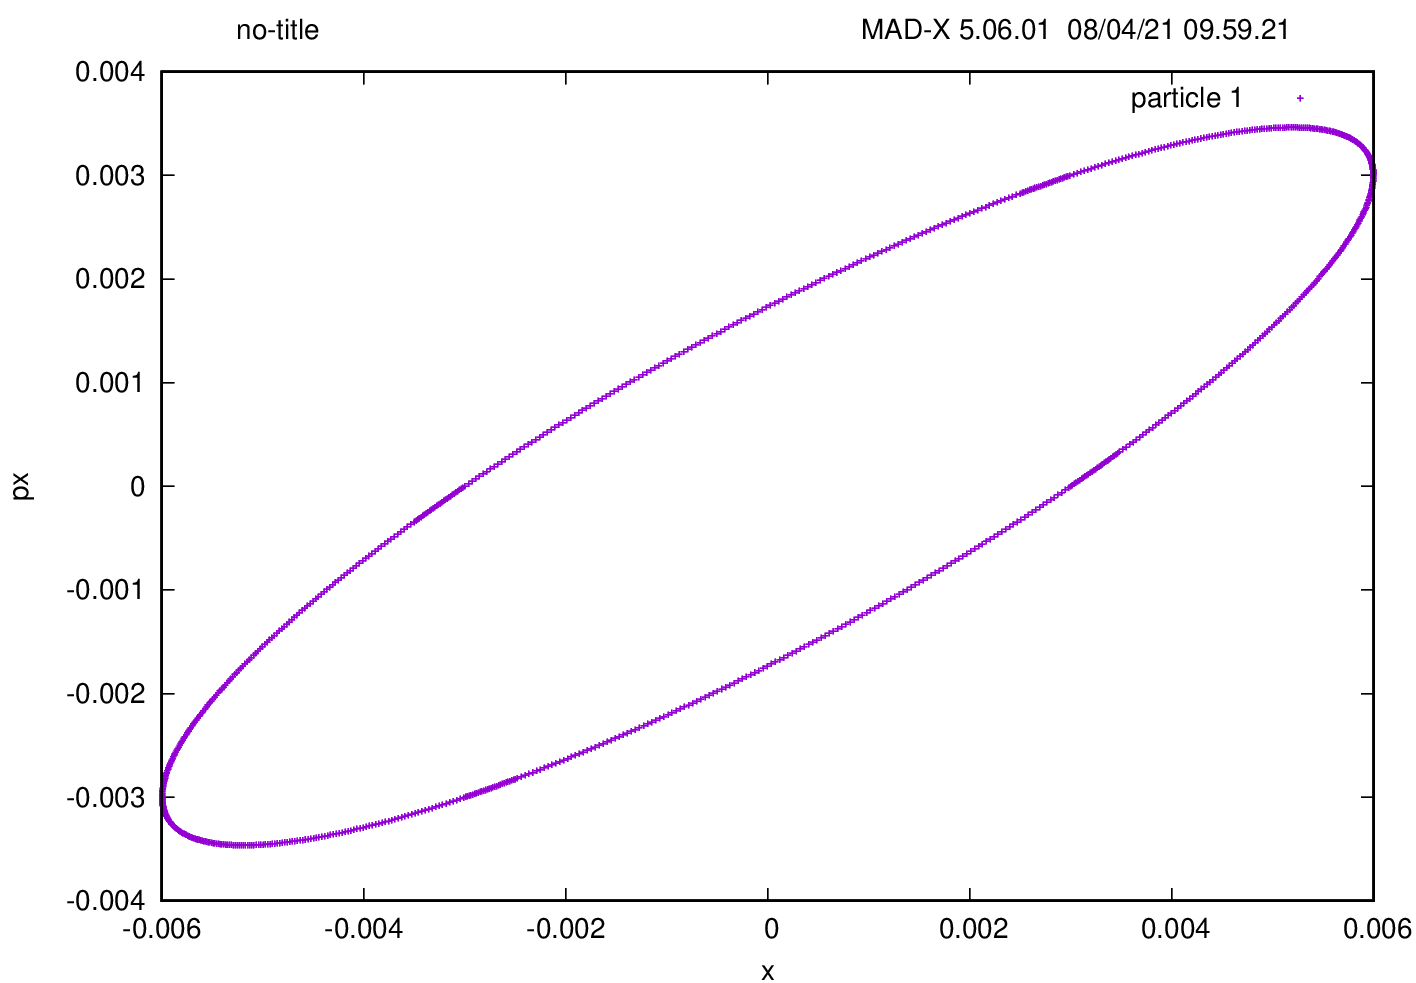
\includegraphics[width=\textwidth]{../../part1/d1f1_x.png}
    \end{minipage}\hfill
    \begin{minipage}{0.49\textwidth}
        \centering
        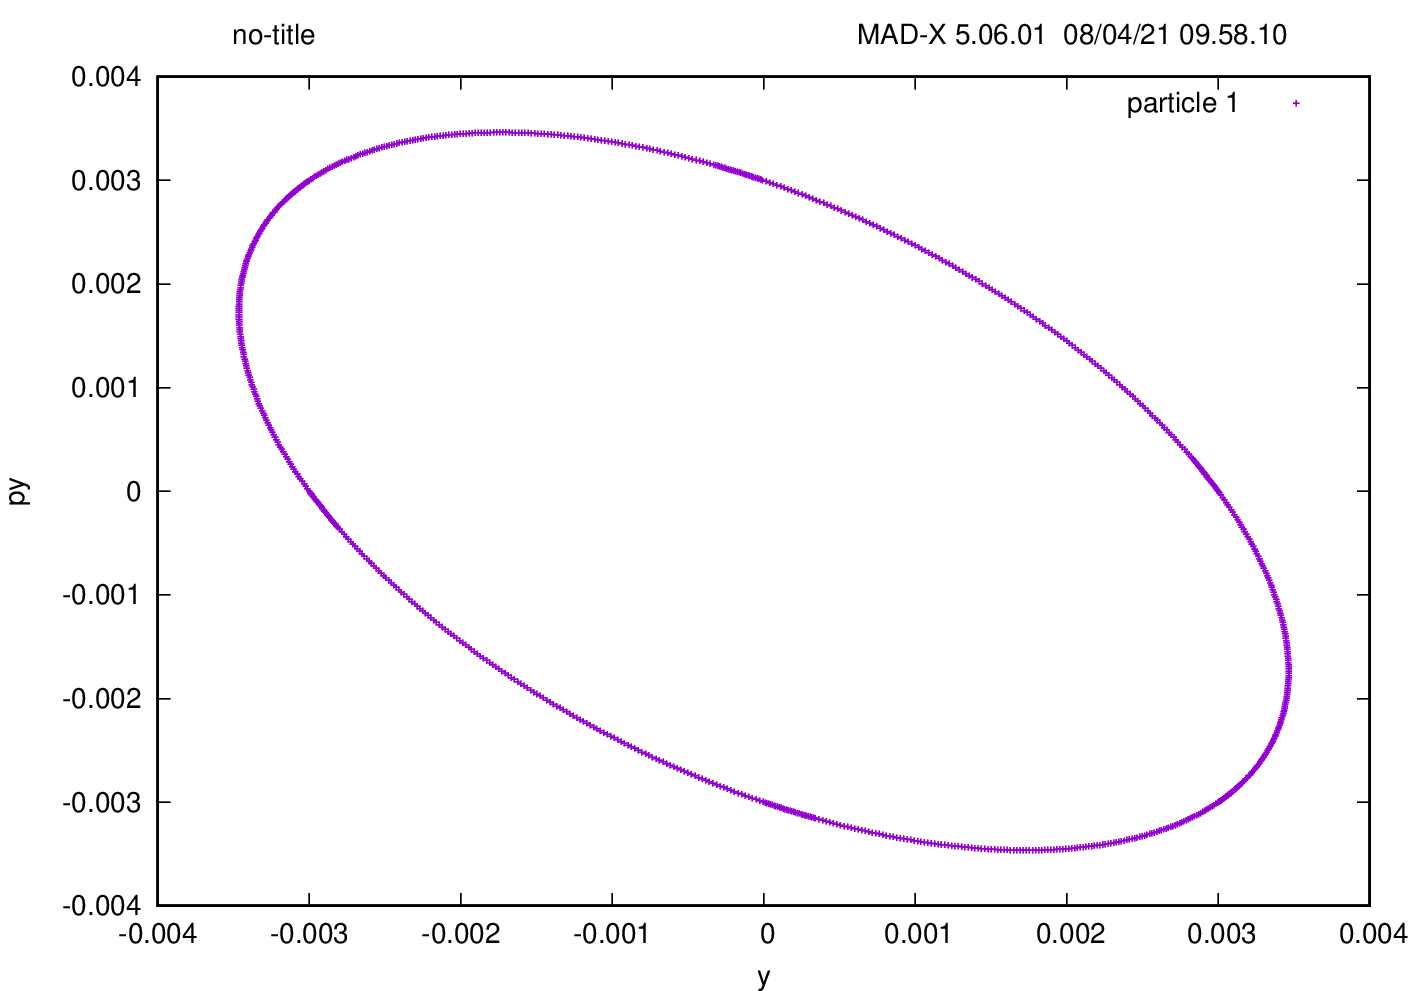
\includegraphics[width=\textwidth]{../../part1/d1f1_y.png}
    \end{minipage}
    \caption{Phase space ellipses for $D=f=1$}
    \label{fig:ellipse}
\end{figure}

Whether a FODO cell is leading to a stable path can be seen from the stability criterion $|D/(2\cdot f)|<1$.
If this inequality is violated, the particle will be lost as can be seen in figure \ref{fig:unstable}
\begin{figure}
    \centering
    \begin{minipage}{0.49\textwidth}
        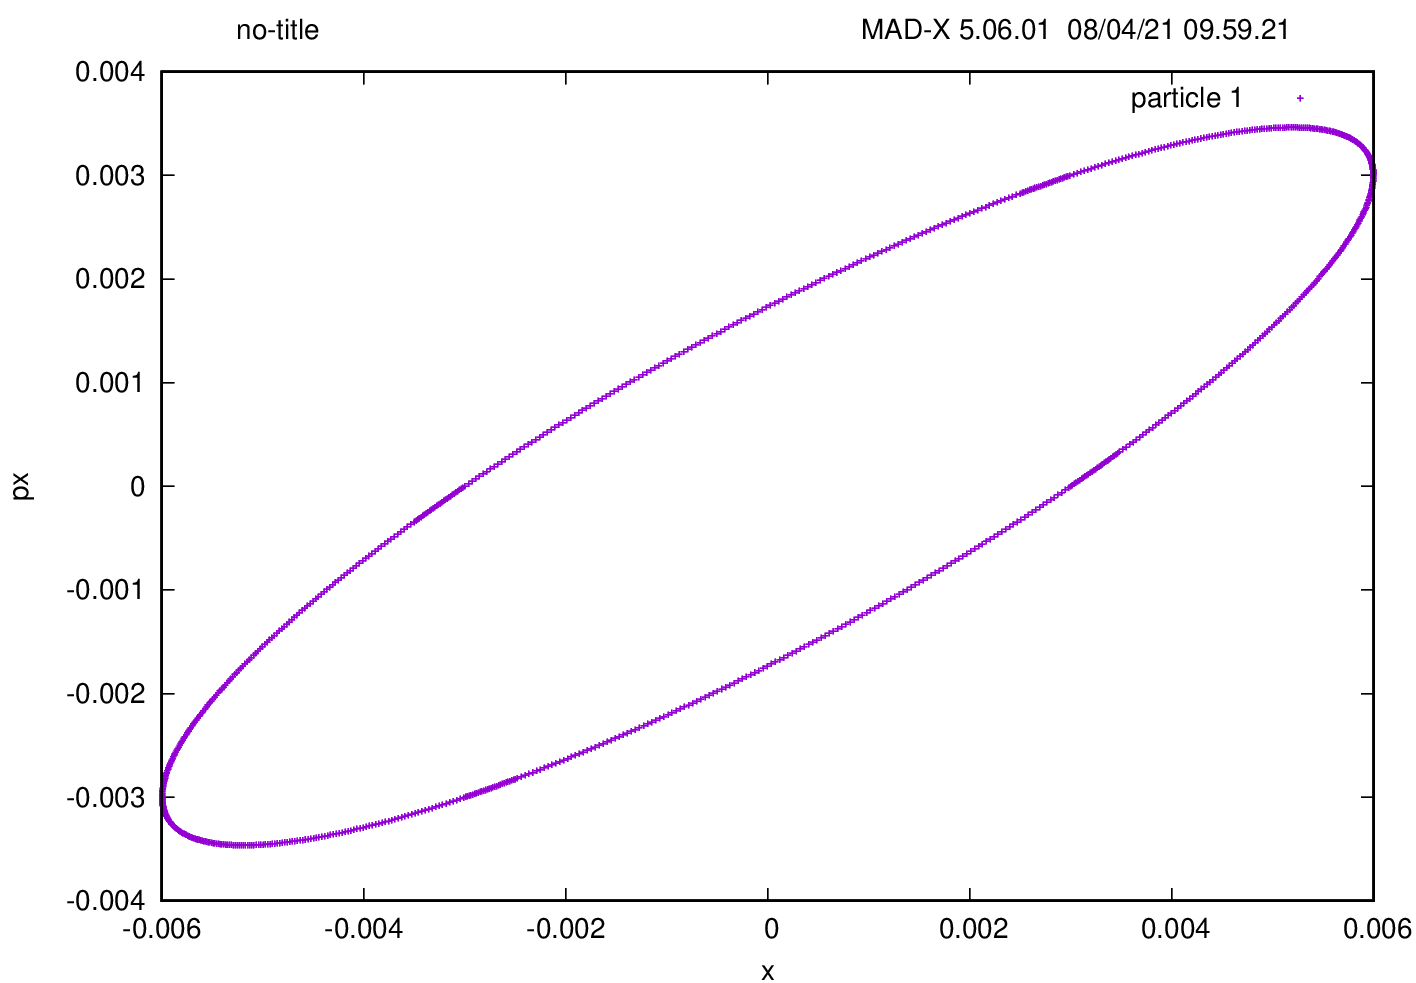
\includegraphics[width=\textwidth]{../../part1/d1f1_x.png}
    \end{minipage}\hfill
    \begin{minipage}{0.49\textwidth}
        \centering
        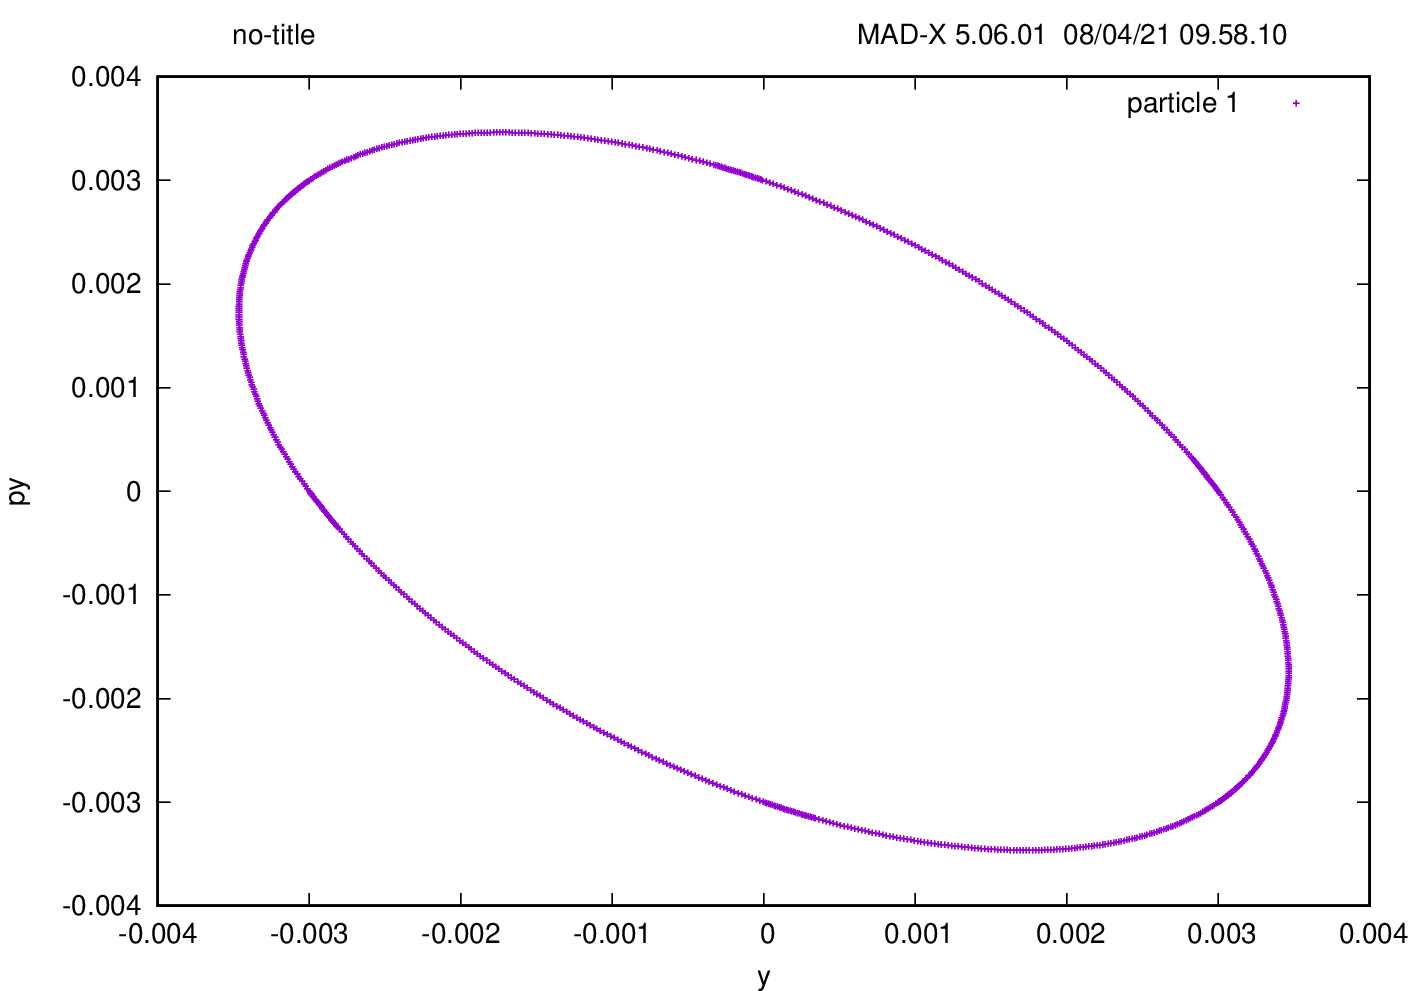
\includegraphics[width=\textwidth]{../../part1/d1f1_y.png}
    \end{minipage}
    \caption{Phase space ellipses for $D=f=1$}
    \label{fig:ellipse}
\end{figure}